\documentclass[a4paper,12pt]{article}
%%%%%%%%%%%%%%%%%%%%%%%%%%%%%%%%%%%%%%%%%%%%%%%%%%%%%%%%%%%%%%%%%%%%%%%%%%%%%%%%%%%%%%%%%%%%%%%%%%%%%%%%%%%%%%%%%%%%%%%%%%%%%%%%%%%%%%%%%%%%%%%%%%%%%%%%%%%%%%%%%%%%%%%%%%%%%%%%%%%%%%%%%%%%%%%%%%%%%%%%%%%%%%%%%%%%%%%%%%%%%%%%%%%%%%%%%%%%%%%%%%%%%%%%%%%%
\usepackage{eurosym}
\usepackage{vmargin}
\usepackage{amsmath}
\usepackage{graphics}
\usepackage{epsfig}
\usepackage{enumerate}
\usepackage{multicol}
\usepackage{subfigure}
\usepackage{fancyhdr}
\usepackage{listings}
\usepackage{framed}
\usepackage{graphicx}
\usepackage{amsmath}
\usepackage{chngpage}
%\usepackage{bigints}

\usepackage{vmargin}
% left top textwidth textheight headheight
% headsep footheight footskip
\setmargins{2.0cm}{2.5cm}{16 cm}{22cm}{0.5cm}{0cm}{1cm}{1cm}
\renewcommand{\baselinestretch}{1.3}

\setcounter{MaxMatrixCols}{10}

\begin{document}

\large 
\noindent A particle is moving on the graph below by starting on a randomly chosen vertex (each with
the same probability) and at each time step moving along one of the adjacent edges to a
neighbouring vertex, choosing the edge with equal probability and independently of all
previous movements.
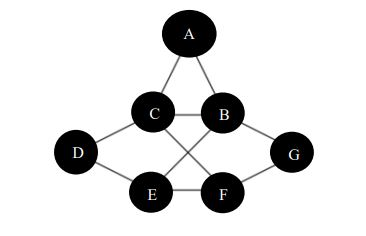
\includegraphics[]{00-B2/images/B2-Q5-Graph.JPG}




%%%%%%%%%%%%%%%%%%%%%%%%%%%%%%
\newpage 
Create a matrix with the transition matrix with probabilities using the state names as
{A,B,C,D,E,F,G} and plot the transition matrix graph. 
\begin{framed}\begin{verbatim}
 #Create a matrix with the transition probabilities.

Matrix2<- matrix(c(
0,1/2,1/2,0,0,0,0,
1/4,0,1/4,0,1/4,0,1/4,
1/4,1/4,0,1/4,0,1/4,0,
0,0,1/2,0,1/2,0,0,
0,1/3,0,1/3,0,1/3,0,
0,0,1/3,0,1/3,0,1/3,
0,1/2,0,0,0,1/2,0),
byrow=TRUE,nrow=7)

Matrix2

\end{verbatim}\end{framed}

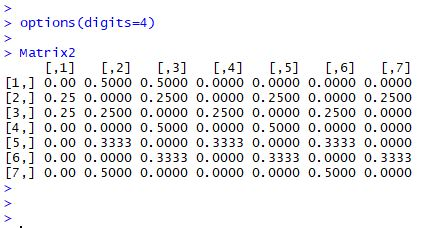
\includegraphics[]{00-B2/images/TransitionMatrix.JPG}


\begin{framed}
sum(Matrix2[1,])
sum(Matrix2[2,])
sum(Matrix2[3,])
sum(Matrix2[4,])
sum(Matrix2[5,])
sum(Matrix2[6,])
sum(Matrix2[7,])
\end{framed}



1




\begin{framed}\begin{verbatim}
#Create a vector with state names
statesmatrix1 <- c("A","B","C","D","E","F","G")
statesmatrix1
\end{verbatim}\end{framed}


<ol class="list-inline">
	<li>'A'</li>
	<li>'B'</li>
	<li>'C'</li>
	<li>'D'</li>
	<li>'E'</li>
	<li>'F'</li>
	<li>'G'</li>
</ol>




\begin{framed}\begin{verbatim}
transitionmat1<-
new("markovchain",
states=statesmatrix1,
transitionMatrix=Matrix2)
\end{verbatim}\end{framed}






> statesmatrix1
[1] "A" "B" "C" "D" "E" "F" "G"
#Create the transition matrix

%%%%%%%%%%%%%%%%%%%%%%%%%%%%%%%%%%


transitionmat1
CS2B-0619
markovchain::plot(transitionmat1)
> transitionmat1
Unnamed Markov chain
A 7 - dimensional discrete Markov Chain defined by the following states:
A, B, C, D, E, F, G
The transition matrix (by rows) is defined as follows:
A
B
C
D
E
F
G


A 0.00 0.5000000 0.5000000 0.0000000 0.0000000 0.0000000 0.0000000
B 0.25 0.0000000 0.2500000 0.0000000 0.2500000 0.0000000 0.2500000
C 0.25 0.2500000 0.0000000 0.2500000 0.0000000 0.2500000 0.0000000
D 0.00 0.0000000 0.5000000 0.0000000 0.5000000 0.0000000 0.0000000
E 0.00 0.3333333 0.0000000 0.3333333 0.0000000 0.3333333 0.0000000
F 0.00 0.0000000 0.3333333 0.0000000 0.3333333 0.0000000 0.3333333
G 0.00 0.5000000 0.0000000 0.0000000 0.0000000 0.5000000 0.0000000


%%%%%%%%%%%%%%%%%%%%%%%%%%%
\newpage 
\subsection*{Exercise 2}
What is the absorbing state in the transition matrix? Find the steady state or stationary
distribution.



ii) # What are the absorbing states?
markovchain::absorbingStates(transitionmat1)
# Find the steady state or stationary distribution.
markovchain::steadyStates(transitionmat1)
> markovchain::steadyStates(transitionmat1)
A B C D E F G
[1,] 0.1 0.2 0.2 0.1 0.15 0.15 0.1





\newpage 
\subsection*{Exercise 3}

How much time it will take to reach the steady state if the particle is starting from state
A, B and C?



iii) # Time to reach steady state if particle starts from A

\begin{verbatim}
n=0
starting=c(1,0,0,0,0,0,0)
while(starting%*%Matrix2!=starting){
starting=starting%*%Matrix2
print(starting)
n=n+1
print(n)
}    
\end{verbatim}

[1] 54
[,1] [,2] [,3] [,4] [,5] [,6] [,7]
[1,] 0.1 0.2 0.2 0.1 0.15 0.15 0.1
[1] 55
There were 50 or more warnings (use warnings() to see the first 50)


%%%%%%%%%%%%%%%%%%%%%%%%%%%%%%%%%
# Time to reach steady state if particle starts from B

\begin{verbatim}
m=0
starting=c(0,1,0,0,0,0,0)
while(starting%*%Matrix2!=starting){
starting=starting%*%Matrix2
print(starting)
m=m+1
print(m)
}    
\end{verbatim}

[1,] 0.1 0.2007407 0.1992593 0.1004772 0.1492593 0.1507407 0.09952283
[1] 54
There were 50 or more warnings (use warnings() to see the first 50)
# Time to reach steady state if particle starts from C

\begin{framed}
\begin{verbatim}
p=0
starting=c(0,0,1,0,0,0,0)

while(starting%*%Matrix2!=starting){
    starting=starting%*%Matrix2
    print(starting)
    p=p+1
    print(p))
}    
\end{verbatim}
\end{framed}
[1,] 0.1 0.1993928 0.2006072 0.09960879 0.1506072 0.1493928 0.1003912
[1] 56
There were 50 or more warnings (use warnings() to see the first 50)
\end{document}
